\chapter{Modelo de Casos de Uso}
\label{sec-casos-de-uso}
\vspace{-1cm}

% Define contador e identificador para casos de uso.
% Usar \UC\label{rf-nome-do-label} para cada caso de uso definido.
\newcounter{uccount}
\renewcommand*\theuccount{UC-\arabic{uccount}}
\newcommand*\UC{\refstepcounter{uccount}\theuccount}
\setcounter{uccount}{0}

\vitor{Listar e descrever os atores na Tabela~\ref{tbl-casos-de-uso-atores}. Criar uma subseção para cada subsistema e, dentro dela, apresentar o diagrama de casos de uso (ex.: Figura~\ref{fig-casos-de-uso-subsistema-01}), a tabela de casos de uso cadastrais (ex.: Tabela~\ref{tbl-casos-de-uso-subsistema-01-cruds}), a tabela de casos de uso de consulta (ex.: Tabela~\ref{tbl-casos-de-uso-subsistema-01-consultas}) e, por fim, a descrição dos demais casos de uso, uma por página (ex.: \ref{uc-subsistema-01-exemplo-05}). As tabelas possuem instruções e exemplos de como devem ser preenchidas.}

O modelo de casos de uso corresponde a uma tentativa de descrever a relação das funcionalidades do sistema com cada um de seus atores. Os atores identificados no contexto deste projeto estão descritos na Tabela~\ref{tbl-casos-de-uso-atores}.

% Tabela de atores.
\begin{longtable}{|p{3cm}|p{12cm}|}
	\caption{Descrição dos atores envolvidos nos casos de uso.}
	\label{tbl-casos-de-uso-atores} \\\hline 
	
	% Cabeçalho e repetição do mesmo em cada nova página. Manter como está.
	\rowcolor{lightgray}
	\textbf{Ator} & \textbf{Descrição} \\\hline		
	\endfirsthead
	\hline
	\rowcolor{lightgray}
	\textbf{Ator} & \textbf{Descrição} \\\hline		
	\endhead
	
	% Especificar os atores abaixo, substituindo os exemplos.
	Ator 01 & Descrição do ator 01. \\\hline
	
	Ator 02 & Descrição do ator 02. \\\hline
	
	Ator 03 & Descrição do ator 03. \\\hline
\end{longtable}

A seguir, são apresentados os diagramas de casos de uso e descrições associadas, organizados por subsistema.



% Definir uma subseção para cada subsistema.	
\section{Subsistema 01}
\label{sec-casos-de-uso-subsistema-01}

A Figura~\ref{fig-casos-de-uso-subsistema-01} apresenta o diagrama de casos de uso do subsistema 01.

\begin{figure}
	\centering
	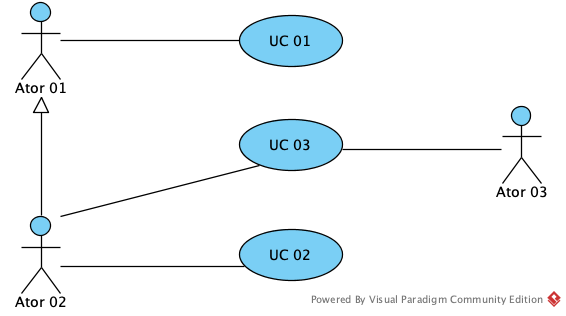
\includegraphics[width=.7\textwidth]{figuras/fig-casos-de-uso-subsistema-01.png}
	\caption{Diagrama de Casos de Uso do subsistema 01.}
	\label{fig-casos-de-uso-subsistema-01}
\end{figure}

A seguir, são apresentadas as descrições de cada um dos casos de uso identificados. Os casos de uso cadastrais de baixa complexidade, envolvendo inclusão, consulta, alteração e exclusão (CRUDs), são descritos na Tabela~\ref{tbl-casos-de-uso-subsistema-01-cruds}.

% Tabela de casos de uso cadastrais.
\begin{longtable}{|c|p{2.5cm}|p{6cm}|p{2.2cm}|p{2cm}|}
	\caption{Caso de uso cadastrais do subsistema 01.}
	\label{tbl-casos-de-uso-subsistema-01-cruds} \\\hline 
	
	% Cabeçalho e repetição do mesmo em cada nova página. Manter como está.
	\rowcolor{lightgray}
	\textbf{Id} & \textbf{Nome} & \textbf{Ações} & \textbf{Requisitos} & \textbf{Classes} \\\hline	
	\endfirsthead
	\hline
	\rowcolor{lightgray}
	\textbf{Id} & \textbf{Nome} & \textbf{Ações} & \textbf{Requisitos} & \textbf{Classes} \\\hline	
	\endhead
	
	% Especificar os atores abaixo, substituindo os exemplos.
	\UC\label{uc-subsistema-01-exemplo-01} & Caso de uso 01 & 
		\begin{itemize}[nosep,leftmargin=8mm]\vspace{-6mm}
			\item[(I)] Restrições de Inclusão;
			\item[(C)] Consulta;
			\item[(A)] Alteração;
			\item[(E)] e Exclusão.
		\vspace{-4mm}\end{itemize}
		& Listar os requisitos satisfeitos por este UC. 
		& Listar possíveis classes envolvidas.
		\\\hline

	\UC\label{uc-subsistema-01-exemplo-02} & Caso de uso 02 & 
		\begin{itemize}[nosep,leftmargin=8mm]\vspace{-6mm}
			\item[(I)] Sem restrições;
			\item[(C)] Sem restrições;
			\item[(A)] Atributos X, Y, Z não podem ser alterados;
			\item[(E)] Não disponível.
		\vspace{-4mm}\end{itemize}
		& \ref{rf-exemplo-01}, \ref{rf-exemplo-02}
		& Classe 01, Classe 02.
		\\\hline
\end{longtable}

Os casos de uso de consulta mais abrangente que as consultas a um único objeto, mas ainda de baixa complexidade, tais como consultas que combinam informações de vários objetos envolvendo filtros, estão descritos na Tabela~\ref{tbl-casos-de-uso-subsistema-01-consultas}.

% Tabela de casos de uso de consulta.
\begin{longtable}{|c|p{2.5cm}|p{6cm}|p{2.2cm}|p{2cm}|}
	\caption{Caso de uso de consultas envolvendo múltiplos objetos do subsistema 01.}
	\label{tbl-casos-de-uso-subsistema-01-consultas} \\\hline 
	
	% Cabeçalho e repetição do mesmo em cada nova página. Manter como está.
	\rowcolor{lightgray}
	\textbf{Id} & \textbf{Nome} &  \textbf{Descrição} & \textbf{Requisitos} & \textbf{Classes} \\\hline	
	\endfirsthead
	\hline
	\rowcolor{lightgray}
	\textbf{Id} & \textbf{Nome} &  \textbf{Descrição} & \textbf{Requisitos} & \textbf{Classes} \\\hline	
	\endhead
	
	% Especificar os atores abaixo, substituindo os exemplos.
	\UC\label{uc-subsistema-01-exemplo-03} & Caso de uso 03 & Descrição da consulta a ser realizada. & Listar os requisitos satisfeitos por este UC. & Listar possíveis classes envolvidas. \\\hline
	
	\UC\label{uc-subsistema-01-exemplo-04} & Caso de uso 04 & Descrição da consulta a ser realizada. & \ref{rf-exemplo-03} & Classe 03, Classe 04. \\\hline
\end{longtable}

Os casos de uso deste subsistema que não se encaixam nas categorias acima são descritos nas páginas subsequentes.


% Descrição de um caso de uso. 
% Reproduzir quantas forem necessárias para descrever os casos de uso que não se encaixarem como CRUDs ou consultas.
\clearpage
\begin{center}\textbf{Descrição de Caso de Uso}\end{center}

\noindent\textbf{Projeto:} \imprimirtitulo \\
\textbf{Identificador:} \UC\label{uc-subsistema-01-exemplo-05} \\
\textbf{Nome:} Caso de uso 05 \\
\textbf{Descrição:} descrição sucinta do propósito deste caso de uso.\\

% Tabela de descrição de um caso de uso.
\begin{longtable}{|p{2.3cm}|p{2.5cm}|p{10cm}|}
	\caption{Fluxos de eventos normais para o caso de uso 05.}
	\label{tbl-casos-de-uso-subsistema-01-exemplo-05} \\\hline 
	
	% Cabeçalho e repetição do mesmo em cada nova página. Manter como está.
	\rowcolor{lightgray}
	Cenário & Precondição & Descrição \\\hline	
	\endfirsthead
	\hline
	\rowcolor{lightgray}
	Cenário & Precondição & Descrição \\\hline
	\endhead
	
	% Especificar os cenários abaixo, substituindo os exemplos.
	Cenário 01 & Precondição do cenário 01 & 
	\begin{enumerate}[nosep,leftmargin=8mm]\vspace{-6mm}
			\item O ator faz algo;
			\item O sistema responde de certa forma;
			\item O ator reage de um jeito;
			\item O sistema etc...
	\vspace{-4mm}\end{enumerate} \\\hline

	Cenário 02 & Precondição do cenário 02 & 
	\begin{enumerate}[nosep,leftmargin=8mm]\vspace{-6mm}
		\item O ator faz algo;
		\item O sistema responde de certa forma;
		\item O ator reage de um jeito;
		\item O sistema etc...
	\vspace{-4mm}\end{enumerate} \\\hline
\end{longtable}


\noindent\textbf{Fluxos variantes:}\vspace{-4mm}
\begin{itemize}
	\item No \textbf{cenário 01}, no caso de \textbf{isso ou aquilo acontecer}, o sistema deve ...
\end{itemize}

\noindent\textbf{Requisitos relacionados:} \ref{rf-exemplo-01}, \ref{rf-exemplo-03}

\noindent\textbf{Classes relacionadas:} \hl{listar possíveis classes relacionadas}.
\newpage


% Definir uma subseção para cada subsistema.	
\section{Subsistema 02}
\label{sec-casos-de-uso-subsistema-02}

Etc...

